\chapter{Конструкторская часть}

\section{Требования к программе}

К разрабатываемому программному обеспечению предъявляется следующий набор функциональных требований:
\begin{enumerate}
	\item программное обеспечение должно предоставлять пользователю текстовый интерфейс для выбора режима работы;
	\item необходимо реализовать поддержку двух основных режимов:
	      \begin{itemize}
		      \item умножение двух матриц с ручным вводом данных;
		      \item массовое тестирование для замера производительности на матрицах различных размеров.
	      \end{itemize}
	\item в ручном режиме программа должна запрашивать размеры и элементы двух исходных матриц, выполнять валидацию вводимых данных (размеры должны быть положительными числами) и проверять совместимость матриц для операции умножения;
	\item в режиме массового тестирования должны выполняться замеры процессорного времени для каждого из реализованных алгоритмов. Результаты замеров следует выводить в наглядном табличном формате.
\end{enumerate}

\section{Разработка алгоритмов}

Визуальное представление логики работы алгоритмов представлено в виде блок-схем. На рисунке~\ref{fig:std_scheme} показана схема стандартного алгоритма. Схема алгоритма Винограда показана на рисунках~\ref{fig:vino_scheme_1} и~\ref{fig:vino_scheme_2}.
Схема оптимизированного алгоритма Винограда представлена на рисунках~\ref{fig:opt_vino_scheme_1} и~\ref{fig:opt_vino_scheme_2}.

\begin{figure}[h!]
	\centerline{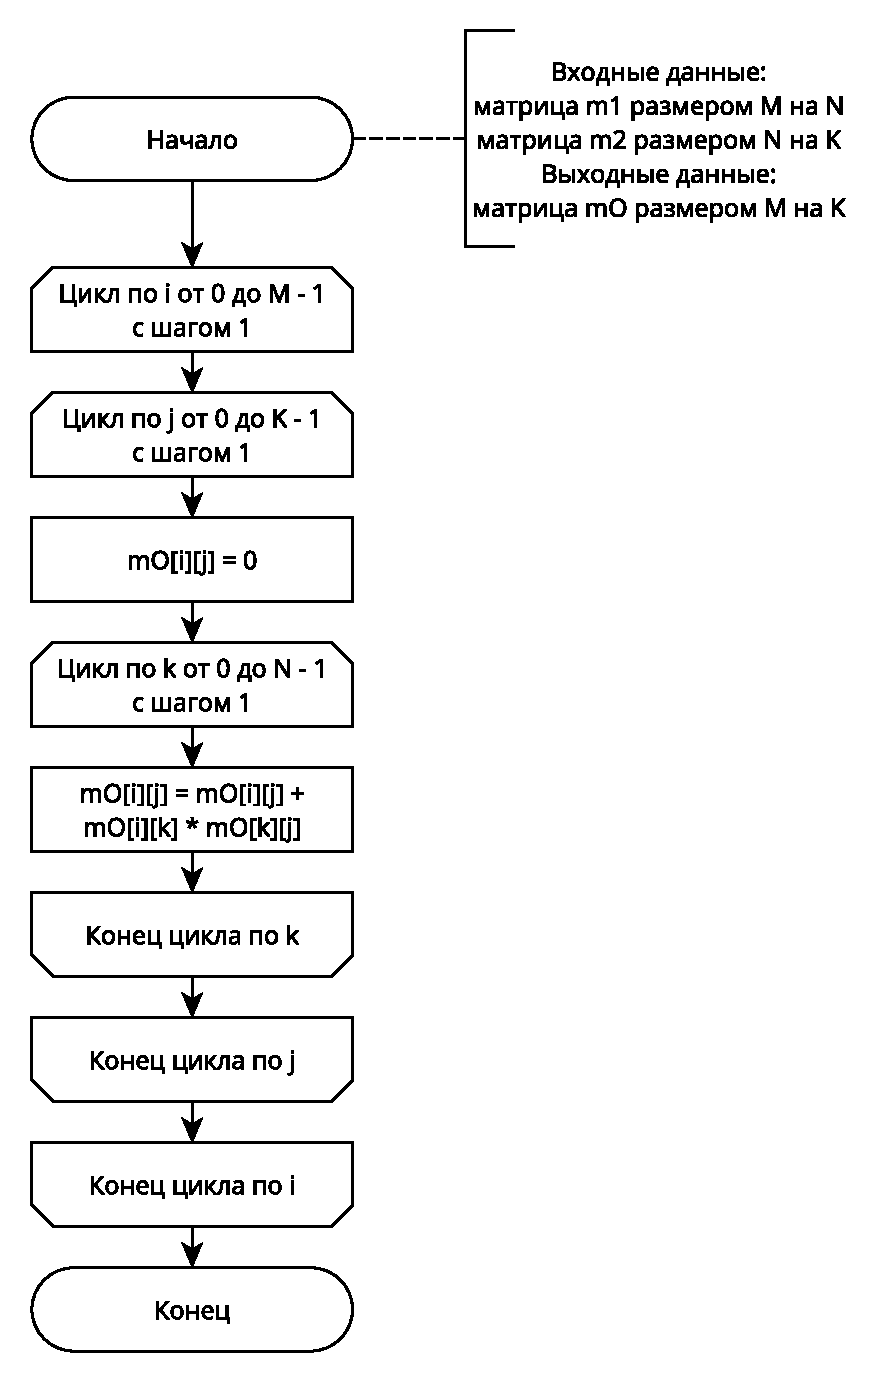
\includegraphics[height=18cm]{images/std_scheme}}
	\caption{Схема стандартного алгоритма умножения матриц}
	\label{fig:std_scheme}
\end{figure}

\begin{figure}[h!]
	\centerline{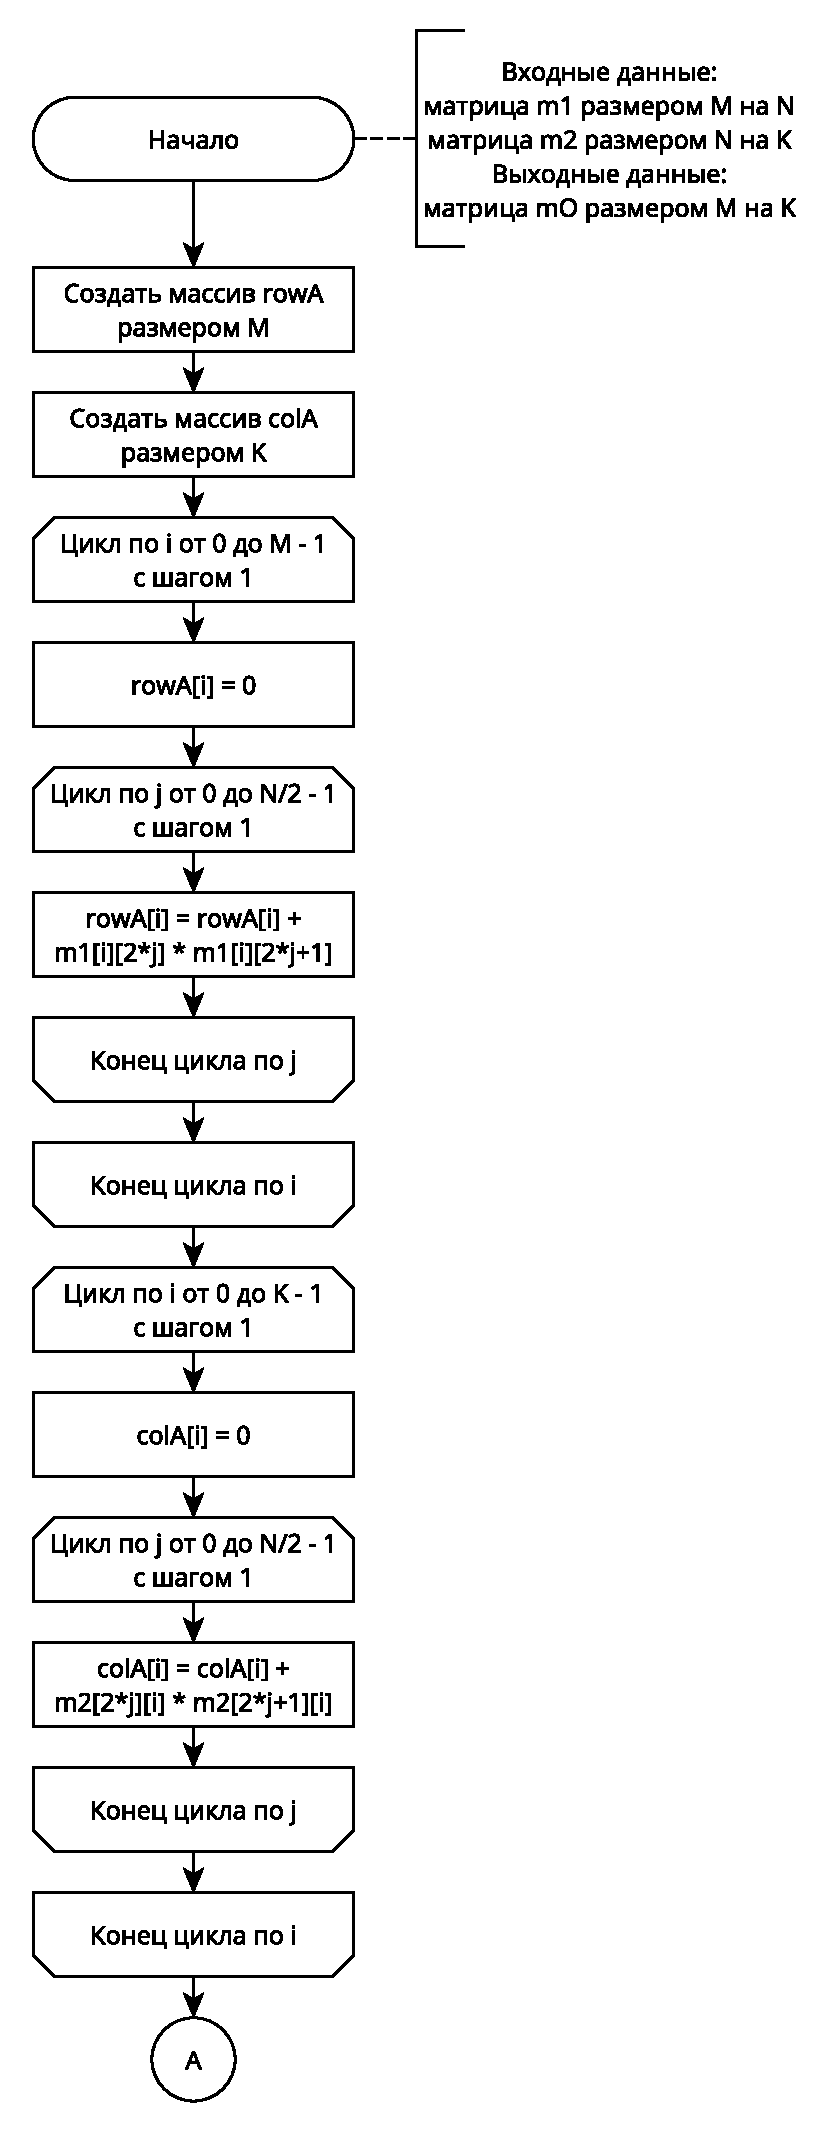
\includegraphics[height=24cm]{images/vino_scheme_1}}
	\caption{Схема алгоритма Винограда (часть 1)}
	\label{fig:vino_scheme_1}
\end{figure}

\begin{figure}[h!]
	\centerline{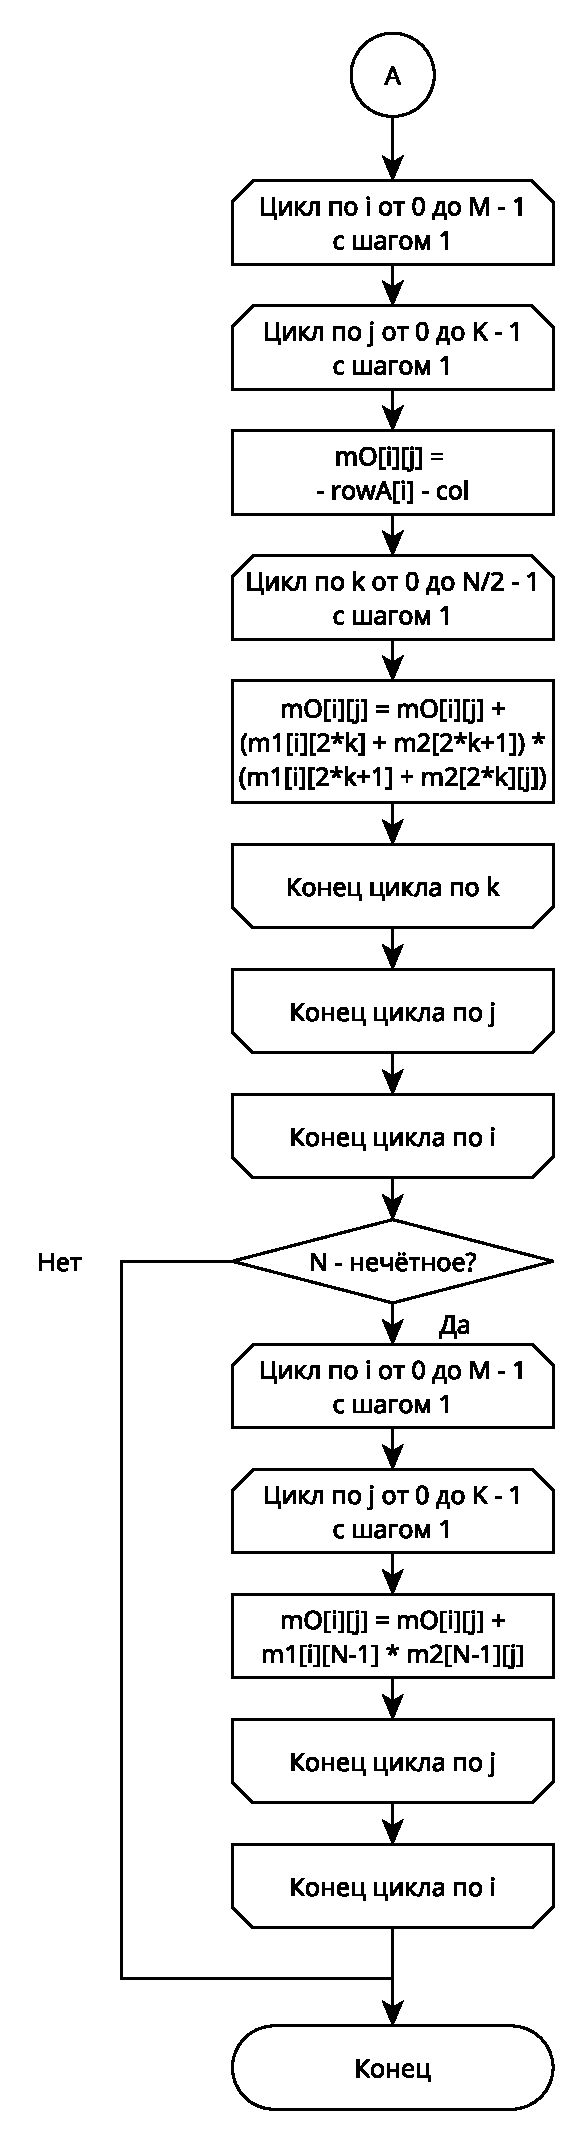
\includegraphics[height=24cm]{images/vino_scheme_2}}
	\caption{Схема алгоритма Винограда (часть 2)}
	\label{fig:vino_scheme_2}
\end{figure}

\begin{figure}[h!]
	\centerline{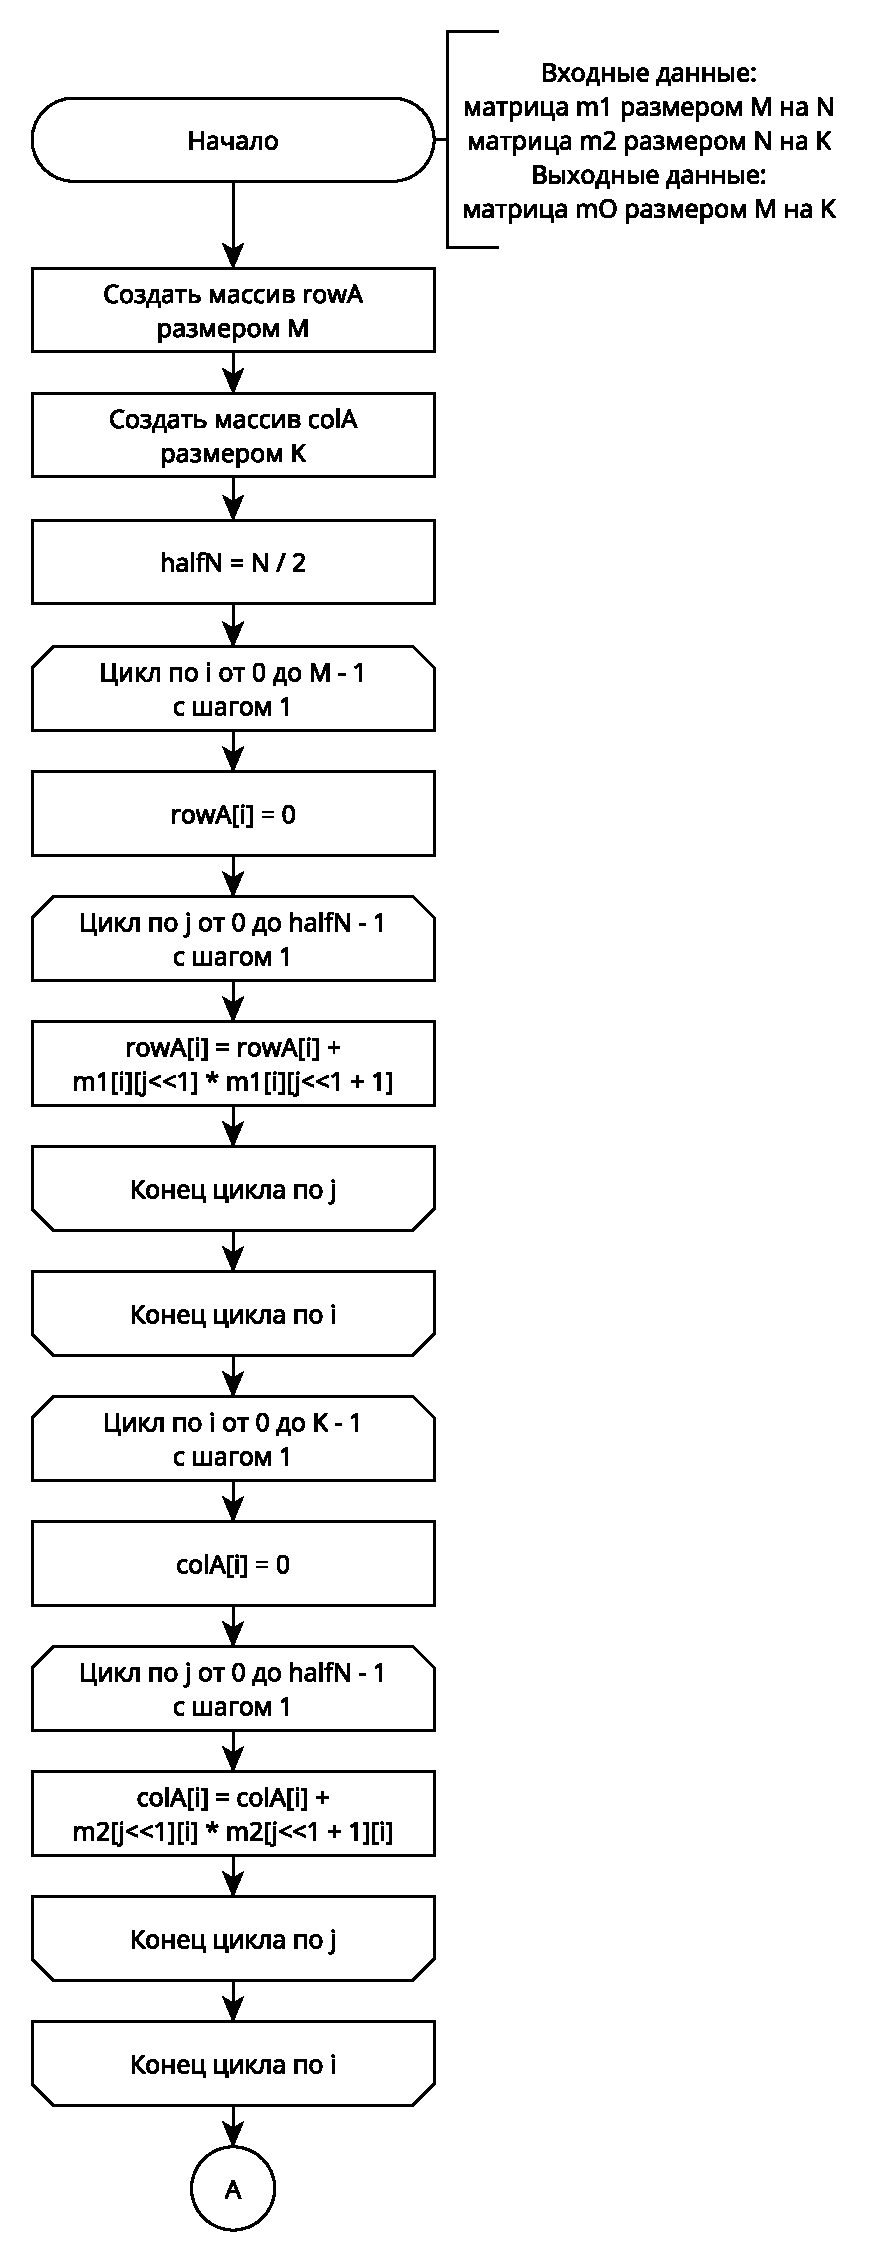
\includegraphics[height=24cm]{images/vino_opt_scheme_1}}
	\caption{Схема оптимизированного алгоритма Винограда (часть 1)}
	\label{fig:opt_vino_scheme_1}
\end{figure}

\begin{figure}[h!]
	\centerline{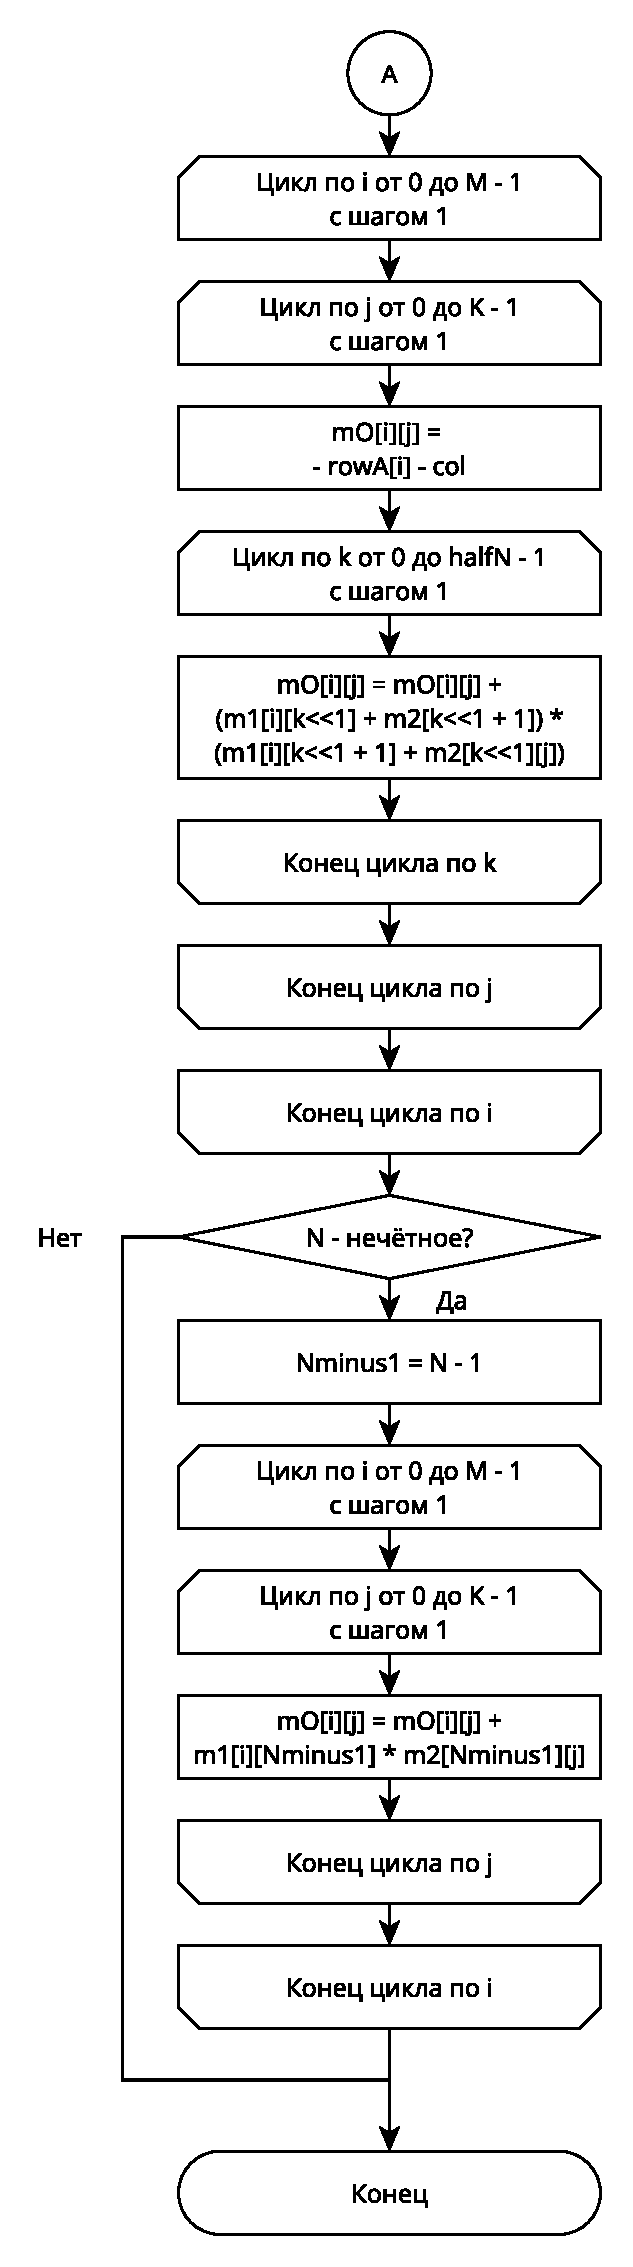
\includegraphics[height=24cm]{images/vino_opt_scheme_2}}
	\caption{Схема оптимизированного алгоритма Винограда (часть 2)}
	\label{fig:opt_vino_scheme_2}
\end{figure}
\clearpage

\section{Модель вычислений}

Для проведения теоретического анализа и оценки трудоёмкости алгоритмов вводится следующая модель вычислений:
\begin{enumerate}
	\item стоимость базовых операций. Операции присваивания, сравнения, инкремента/декремента, простого сложения/вычитания и индексации массива ($=, ==, !=, <, >, <=, >=, ++, --, +, -, []$) имеют условную стоимость, равную 1;
	\item стоимость арифметических операций. Операции умножения, деления и взятия остатка ($\cdot, /, \%$) считаются более затратными и имеют условную стоимость, равную 2;
	\item трудоёмкость условного оператора. Для оператора \textit{if (условие)} \{блок X\} \textit{else} \{блок Y\} общая трудоёмкость ($f_{\text{if}}$) складывается из стоимости вычисления условия ($f_{\text{условия}}$) и стоимости выполнения соответствующей ветви:
	      \begin{equation}
		      \label{eq:if_cost}
		      f_{\text{if}} = f_{\text{условия}} +
		      \begin{cases}
			      \min(f_X, f_Y), & \text{в лучшем случае} \\
			      \max(f_X, f_Y), & \text{в худшем случае}
		      \end{cases}
	      \end{equation}
	\item трудоёмкость цикла. Для цикла \textit{for} с $M$ итерациями общая трудоёмкость ($f_{\text{for}}$) рассчитывается как сумма стоимости инициализации ($f_{\text{init}}$), всех проверок условия ($M+1$ раз) и выполнения тела цикла и инкремента ($M$ раз):
	      \begin{equation}
		      \label{eq:for_cost}
		      f_{\text{for}} = f_{\text{init}} + (M+1) \cdot f_{\text{условия}} + M \cdot (f_{\text{тело}} + f_{\text{инкремент}})
	      \end{equation}
\end{enumerate}

\section{Расчёт трудоёмкости алгоритмов}

На основе принятой модели вычислений проведём оценку теоретической трудоёмкости для каждого из алгоритмов. Пусть матрицы имеют размеры $M \times N$ и $N \times K$.

\subsection{Стандартный алгоритм}
Трудоёмкость стандартного алгоритма определяется тремя вложенными циклами. Применив формулу \eqref{eq:for_cost}, получается итоговую оценку:
\begin{equation}
	f_{\text{std}} = 2 + M \cdot (2 + K \cdot (5 + N \cdot (2+12))) = 14MNK + 5MK + 2M + 2 \approx 14MNK
	\label{eq:std_complexity}
\end{equation}

\subsection{Алгоритм Винограда}
Общая трудоёмкость складывается из четырёх этапов: вычисление факторов строк ($f_1$), факторов столбцов ($f_2$), основной цикл ($f_3$) и коррекция для нечётного случая ($f_{\text{if}}$).
\begin{enumerate}
	\item заполнение \textit{row\_factor}: $f_1 = 2 + M \cdot (8 + \frac{N}{2} \cdot 19) = \frac{19}{2}MN + 8M + 2$;
	\item заполнение \textit{col\_factor}: $f_2 = 2 + K \cdot (8 + \frac{N}{2} \cdot 19) = \frac{19}{2}NK + 8K + 2$;
	\item основной цикл: $f_3 = 2 + M \cdot (4 + K \cdot (13 + \frac{N}{2} \cdot 32)) \approx 16MNK$;
	\item коррекция для нечётного $N$: $f_{\text{if}}$ в худшем случае составляет $16MK + 4M + 5$.
\end{enumerate}
Итоговая трудоёмкость в худшем случае (нечётное $N$) составляет:
\begin{equation}
	f_{\text{total\_vino}} = 16MNK + 29MK + \frac{19}{2}(MN+NK) + 16M + 8K + 11 \approx 16MNK
	\label{eq:vino_complexity}
\end{equation}

\subsection{Оптимизированный алгоритм Винограда}

\begin{enumerate}
	\item предрасчет \textit{halfN}: $f_0 = 3$;
	\item заполнение \textit{row\_factor}: $f_1 = 2 + M \cdot (6 + \frac{N}{2} \cdot 17) = \frac{17}{2}MN + 6M + 2$;
	\item заполнение \textit{col\_factor}: $f_2 = 2 + K \cdot (6 + \frac{N}{2} \cdot 17) = \frac{17}{2}NK + 6K + 2$;
	\item основной цикл: $f_3 = 2 + M \cdot (4 + K \cdot (11 + \frac{N}{2} \cdot 26)) \approx 13MNK$;
	\item коррекция для нечётного $N$: $f_{\text{if}}$ в худшем случае составляет $14MK + 4M + 6$.
\end{enumerate}
Итоговая трудоёмкость в худшем случае (нечётное $N$) составляет:
\begin{equation}
	f_{\text{total\_vino}} = 13MNK + 27MK + \frac{17}{2}(MN+NK) + 14M + 6K + 15 \approx 13MNK
	\label{eq:vino_opt_complexity}
\end{equation}


\section*{Вывод}

В конструкторской части были сформулированы требования к программной реализации и представлены блок-схемы, описывающие логику работы трёх алгоритмов умножения матриц. Была введена модель вычислений, на основе которой проведён теоретический анализ трудоёмкости.

Результаты анализа показывают, что алгоритм Винограда имеет большую трудоёмкость по сравнению со стандартным алгоритмом, а его оптимизированная версия имеют преимущество перед стандартным методом.

\clearpage
